\theme
\renewcommand{\leftmark}{CORRIGÉ DES ACTIVITÉS}
\label{CDA}

\begin{center}
    \rule{\linewidth}{4pt} \par \vskip-3mm
    \rule{\linewidth}{2pt} \par \vskip4pt
    {\Huge\sffamily\bf Corrigé des activités} \par %\vskip8mm
    \rule{\linewidth}{2pt} \par \vskip-2.8mm
    \rule{\linewidth}{4pt}
\end{center}

\ARtitre{Séquence 01 : Nombres en cases} %%%1

    \begin{center}    
        \CalculsCroises[Largeur=22pt,Couleur=RoyalBlue!50]{%
            5,+,1,*,7,%
            *,-,+,%
            6,*,4,*,9,%
            +,-,*,%
            3,+,2,*,8}
        \quad
        \CalculsCroises[Largeur=22pt,ListeNombres={5,4,8},Solution,CouleurS=RoyalBlue]{%
            9,-,4,*,2,%
            *,+,+,%
            5,*,1,+,7,%
            +,*,*,%
            3,*,6,-,8}
    \end{center}
 
    \smallskip

    \begin{center}
        \Garam[Largeur=7mm,Solution,CouleurSolution=RoyalBlue]{%
            !4/+/x,5/=/,!9//+,*,!3/+/x,1/=/,!4//x
            §6//=,*,!4/+/=,4/=/,!8//=,*,5//=
            §2//,*,1//,*,2//,*,!2//
            §4/-/,!1/=/-,!3//,*,!4/-/,!4/=/+,!0//
            §*,1//=,*,*,*,3//=,*
            §!8/-/x,0/=/,8//x,*,9/-/x,!7/=/,!2//x
            §4//=,*,!3/+/=,1/=/,!4//=,*,7//=
            §!3//,*,2//,*,!3//,*,1//
            §!2/+/,2/=/,!4//,*,!6/-/,2/=/,!4//}
        \qquad
        \Garam[Largeur=7mm,Solution,CouleurSolution=RoyalBlue]{%
            !5/+/x,2/=/,!7//x,*,!8/+/x,!0/=/,!8//x
            §5//=,*,!2/+/=,6/=/,!8//=,*,5//=
            §2//,*,1//,*,6//,*,!4//
            §!5/-/,!1/=/+,4//,*,4/-/,!4/=/-,!0//
            §*,2//=,*,*,*,3//=,*
            §!2/+/x,!3/=/,!5//x,*,3/-/x,!1/=/,!2//x
            §7//=,*,!2/+/=,3/=/,!5//=,*,9//=
            §1//,*,!1//,*,1//,*,1//
            §!4/-/,4/=/,!0//,*,!5/+/,3/=/,!8//}
    \end{center}

\vfill


\AAtitre{Séquence 02 : Couples d'angles}

    On peut observer \cor{huit angles différents}.
    \begin{enumerate}
        \item[2.] Il y a \cor{deux paires d'angles alternes-internes} dans cette configuration.
        \item[4.] En théorie, chaque binôme doit trouver la même mesure pour les deux angles.
        \item[6.] Il y a \cor{deux paires d'angles alternes-internes} dans cette configuration.
        \item[8.] En théorie, chaque binôme doit trouver la même mesure pour les deux angles.
    \end{enumerate}

\pagebreak


\AAtitre{Séquence 03 : La fourmi de Langton} %%%3

    \begin{center}
        \psset{unit=0.6,subgriddiv=1,gridlabels=0mm,gridcolor=gray,fillstyle=solid,fillcolor=darkgray}
        \small
            \begin{pspicture}(0,-1.5)(7,7)
                \psgrid(0,0)(7,7)
                \fourmi{3.5}{3.5}{0}
                \rput(3.5,-0.5){étape 0}
            \end{pspicture}
            \quad
            \begin{pspicture}(0,-1.5)(7,7)
                \psframe(3,3)(4,4)
                \psgrid(0,0)(7,7)
                \fourmi{4.5}{3.5}{-90}
                \rput(3.5,-0.5){étape 1}
            \end{pspicture}
            \quad
            \begin{pspicture}(0,-1.5)(7,7)  
                \psframe(3,3)(5,4)
                \psgrid(0,0)(7,7)
                \fourmi{4.5}{2.5}{180}
                \rput(3.5,-0.5){étape 2}
            \end{pspicture}
            \quad
            \begin{pspicture}(0,-1.5)(7,7)
                \psframe[fillcolor=RoyalBlue](3,3)(5,4)
                \psframe[fillcolor=RoyalBlue](4,2)(5,3)
                \fourmi{3.5}{2.5}{90}
                \psgrid(0,0)(7,7)
                \rput(3.5,-0.5){étape 3}
            \end{pspicture}
            \vskip5mm
            \begin{pspicture}(0,-0.7)(7,7)
                \psframe(3,2)(5,4)
                \psgrid(0,0)(7,7)
                \fourmi{3.5}{3.5}{0}
                \rput(3.5,-0.5){étape 4}
            \end{pspicture}
            \quad
            \begin{pspicture}(0,-0.7)(7,7)
                \pspolygon[fillcolor=RoyalBlue](3,2)(5,2)(5,4)(4,4)(4,3)(3,3)
                \fourmi{2.5}{3.5}{90}
                \psgrid(0,0)(7,7)
                \rput(3.5,-0.5){étape 5}
            \end{pspicture}
            \quad
            \begin{pspicture}(0,-0.7)(7,7)
                \pspolygon[fillcolor=RoyalBlue](3,2)(5,2)(5,4)(4,4)(4,3)(3,3)
                \psframe[fillcolor=RoyalBlue](2,3)(3,4)
                \fourmi{2.5}{4.5}{0}
                \psgrid(0,0)(7,7)
                \rput(3.5,-0.5){étape 6}
            \end{pspicture}
            \quad
            \begin{pspicture}(0,-0.7)(7,7)
                \psframe(2,3)(3,5)
                \pspolygon(3,2)(5,2)(5,4)(4,4)(4,3)(3,3)
                \psgrid(0,0)(7,7)
                \fourmi{3.5}{4.5}{-90}
                \rput(3.5,-0.5){étape 7}
            \end{pspicture}
            \vskip5mm
            \begin{pspicture}(0,-0.7)(7,7)
                \psframe(2,3)(3,5)
                \pspolygon(3,2)(5,2)(5,4)(4,4)(4,3)(3,3)
                \psframe(3,4)(4,5)
                \fourmi{3.5}{3.5}{180}
                \psgrid(0,0)(7,7)
                \rput(3.5,-0.5){étape 8}
            \end{pspicture}
            \quad
            \begin{pspicture}(0,-0.7)(7,7)
                \pspolygon[fillcolor=RoyalBlue](3,2)(5,2)(5,4)(4,4)(4,5)(2,5)(2,3)(3,3)
                \fourmi{2.5}{3.5}{90}
                \psgrid(0,0)(7,7)
                \rput(3.5,-0.5){étape 9}
            \end{pspicture}
            \quad
            \begin{pspicture}(0,-0.7)(7,7)
                \pspolygon[fillcolor=RoyalBlue](3,2)(5,2)(5,4)(4,4)(4,5)(2,5)(2,4)(3,4)
                \fourmi{2.5}{2.5}{180}
                \psgrid(0,0)(7,7)
                \rput(3.5,-0.5){étape 10}
            \end{pspicture}
            \quad
            \begin{pspicture}(0,-0.7)(7,7)
                \pspolygon(2,2)(5,2)(5,4)(4,4)(4,5)(2,5)(2,4)(3,4)(3,3)(2,3)
                \psgrid(0,0)(7,7)
                \rput(3.5,-0.5){étape 11}
                \fourmi{1.5}{2.5}{90}
            \end{pspicture}
            \vskip5mm
            \begin{pspicture}(0,-1)(7,7)
                \pspolygon[fillcolor=RoyalBlue](1,2)(5,2)(5,4)(4,4)(4,5)(2,5)(2,4)(3,4)(3,3)(1,3)
                \fourmi{1.5}{3.5}{0}
                \psgrid(0,0)(7,7)
                \rput(3.5,-0.5){étape 12}
            \end{pspicture}
            \quad
            \begin{pspicture}(0,-1)(7,7)
                \pspolygon[fillcolor=RoyalBlue](1,2)(5,2)(5,4)(4,4)(4,5)(2,5)(2,4)(3,4)(3,3)(2,3)(2,4)(1,4)
                \fourmi{2.5}{3.5}{-90}
                \psgrid(0,0)(7,7)
                \rput(3.5,-0.5){étape 13}
            \end{pspicture}
            \quad
            \begin{pspicture}(0,-1)(7,7)
                \pspolygon[fillcolor=RoyalBlue](1,2)(5,2)(5,4)(4,4)(4,5)(2,5)(2,4)(1,4)
                \fourmi{2.5}{2.5}{180}
                \psgrid(0,0)(7,7)
                \rput(3.5,-0.5){étape 14}
            \end{pspicture}
            \quad
            \begin{pspicture}(0,-1)(7,7)
                \pspolygon[fillcolor=RoyalBlue](1,2)(2,2)(2,3)(3,3)(3,2)(5,2)(5,4)(4,4)(4,5)(2,5)(2,4)(1,4)
                \fourmi{3.5}{2.5}{-90}
                \psgrid(0,0)(7,7)
                \rput(3.5,-0.5){étape 15}
            \end{pspicture} 
    \end{center}

\vfill


\ARtitre{Séquence 03 : Le jeu des dominogrammes}

    On obtient cette suite de dominos : \cor{\ding{40} -- \ding{110} -- \ding{57} -- \ding{52} -- \ding{70} -- \ding{74} -- \ding{87} -- \ding{115}}

\pagebreak


\AAtitre{Séquence 04 : Carrés magiques} %%%4

    \begin{center}
        {\psset{unit=1.7,griddots=50, subgriddiv=0, gridlabels=0}
        \large
        \begin{pspicture}(0,-0.3)(4,4)
            \psgrid(0,0)(3,3)
            \rput(0.5,0.5){4}
            \rput(0.5,1.5){\cor{3}}
            \rput(0.5,2.5){8}
            \rput(1.5,0.5){\cor{9}}
            \rput(1.5,1.5){5}
            \rput(1.5,2.5){\cor{1}}
            \rput(2.5,0.5){2}
            \rput(2.5,1.5){\cor{7}}
            \rput(2.5,2.5){\cor{6}}
            \rput(1.4,3.5){Somme =\;\cor{15}}
        \end{pspicture}
        \begin{pspicture}(-1,-0.3)(3,4)
            \psgrid(0,0)(3,3)
            \rput(0.5,0.5){\cor{6}}
            \rput(0.5,1.5){\cor{21}}
            \rput(0.5,2.5){18}
            \rput(1.5,0.5){\cor{27}}
            \rput(1.5,1.5){15}
            \rput(1.5,2.5){\cor{3}}
            \rput(2.5,0.5){12}
            \rput(2.5,1.5){\cor{9}}
            \rput(2.5,2.5){24}
            \rput(1.4,3.5){Somme =\;\cor{45}}
        \end{pspicture}
        
        \begin{pspicture}(0,-0.3)(4,4)
            \psgrid(0,0)(3,3)
            \rput(0.5,0.5){\cor{6}}
            \rput(0.5,1.5){\cor{1}}
            \rput(0.5,2.5){2}
            \rput(1.5,0.5){\cor{$-1$}}
            \rput(1.5,1.5){3}
            \rput(1.5,2.5){7}
            \rput(2.5,0.5){4}
            \rput(2.5,1.5){\cor{5}}
            \rput(2.5,2.5){\cor{0}}
            \rput(1.4,3.5){Somme =\;\cor{9}}
        \end{pspicture}
        \begin{pspicture}(-1,-0.3)(3,4)
            \psgrid(0,0)(3,3) 
            \rput(0.5,0.5){10}
            \rput(0.5,1.5){\cor{$-5$}}
            \rput(0.5,2.5){\cor{16}}
            \rput(1.5,0.5){\cor{13}}
            \rput(1.5,1.5){7}
            \rput(1.5,2.5){1}
            \rput(2.5,0.5){\cor{$-2$}}
            \rput(2.5,1.5){\cor{19}}
            \rput(2.5,2.5){4}
            \rput(1.4,3.5){Somme =\;\cor{21}}
        \end{pspicture}}
    \end{center} 

\vfill


\ARtitre{Séquence 04 : Nombres croisés}

    \begin{center}
        {\hautab{2.5}
        \begin{tabular}{|>{\columncolor[gray]{.8}}C{0.8}|*{6}{C{0.8}|}}
            \hline
            \rowcolor{gray!40} & a & b & c & d & e & f \\
            \hline
            1 & \textcolor{RoyalBlue}{9} & \cellcolor{black!70} & \textcolor{RoyalBlue}{1} & \textcolor{RoyalBlue}{3} & \cellcolor{black!70} & \textcolor{RoyalBlue}{$-$} \\
            \hline
            2 & \textcolor{RoyalBlue}{1} & \textcolor{RoyalBlue}{2} & \textcolor{RoyalBlue}{0} & \cellcolor{black!70} & \textcolor{RoyalBlue}{$-$} & \textcolor{RoyalBlue}{1} \\
            \hline
            3 & \textcolor{RoyalBlue}{8} & \cellcolor{black!70} & \cellcolor{black!70} & \textcolor{RoyalBlue}{7} & \textcolor{RoyalBlue}{4} & \cellcolor{black!70} \\
            \hline
            4 & \cellcolor{black!70} & \textcolor{RoyalBlue}{$-$} & \textcolor{RoyalBlue}{9} & \cellcolor{black!70} & \cellcolor{black!70} & \textcolor{RoyalBlue}{$-$} \\
            \hline
            5 & \textcolor{RoyalBlue}{$-$} & \textcolor{RoyalBlue}{1} & \cellcolor{black!70} & \textcolor{RoyalBlue}{$-$} & \textcolor{RoyalBlue}{1} & \textcolor{RoyalBlue}{6} \\
            \hline
            6 & \textcolor{RoyalBlue}{3} & \cellcolor{black!70} & \textcolor{RoyalBlue}{4} & \textcolor{RoyalBlue}{2} & \textcolor{RoyalBlue}{1} & \cellcolor{black!70} \\
            \hline
        \end{tabular}}
    \end{center}


\pagebreak

\AAtitre{Séquence 05 : Dessin gradué} %%%5

    \begin{center}
        \DessinGradue[LignesIdentiques=false,Echelle=1.5,EcartVertical=0.85,Solution]
            {0/15/15,
            10/25/15,
            50/65/15,
            15/30/15,
            0/30/30,
            20/50/15,
            0/30/15,
            0/45/15,
            100/115/15,
            0/30/15,
            0/150/15,
            0/60/30,
            0/1.5/15,
            -15/0/15}
            {1/A/8,1/B/9,1/C/12,
            2/D/7,2/E/8,2/F/9,2/G/10,2/H/11,2/I/12,2/J/13,
            3/K/7,3/L/8,3/M/9,3/N/13,3/O/14,
            4/P/8,4/Q/9,4/R/10,4/S /13,4/T/14,
            5/U/22,5/V/24,5/W/26,
            6/X/8,6/ Y/12,
            7/Z/3,7/A'/7,7/B'/9,7/C'/11,
            8/D'/5 ,8/E'/6,8/F'/9,
            9/G'/3,9/H'/7,9/I'/8,
            10/J'/1,10/K'/2,10/L'/8,
            11/M'/5,11/N'/8,
            12/O'/16,12/P'/22,
            13/Q'/1,13/R'/2,13/S'/3,13/ T'/5,13/U'/6,13/V'/7,13/W'/8,13/X'/9,
            14/Y'/0,14/Z'/1,14/A''/4,14/B''/8,14/C''/9}
            {chemin(F,E,L,M,P,K,D,A,C,O,T,W,V,Y,C',P',C '',B'',V',O',W',X',B',X,A'),
            chemin(G,B),
            chemin(H,J,N,I),
            chemin(S,T),
            chemin(Q,R,U ,C'),
            chemin(D',E',L',N',U',T'),
            chemin(F ',I',H'),
            chemin(U',V'),
            chemin(B'',A'',S',M',G',K',R',Z',Y',Q',J',Z,K),
            chemin(Z, G')}
    \end{center}

\vfill
\pagebreak


\ARtitre{Séquence 05 : De curieux dessins}

    \begin{multicols}{2}

        {\psset{unit=0.5}
        \begin{pspicture}(-6,-6)(5,8)
            \psgrid[subgriddiv=0,gridcolor=lightgray,gridlabels=0](0,0)(-5,-6)(5,7)
            \psaxes[labels=none]{->}(0,0)(-5,-6)(5,7)
            \rput(-0.4,-0.4){\scriptsize 0}
            \rput(1,-0.5){\scriptsize 1}
            \rput(-0.5,1){\scriptsize 1}
            \psset{linecolor=RoyalBlue}
            \psline(-3,2)(-3,-5)(3,-5)(3,2)(4,1)(4,2)(0,6)(-4,2)(-4,1)(0,5)(3,2) 
            \psframe(-1,-5)(1,-2)
            \psframe(-2,0)(-1,2)
            \psframe(1,-1)(2,1)
        \end{pspicture}}
        
        {\psset{xunit=0.5}
        \begin{pspicture}(-6,-5)(5,7.5)
            \psgrid[subgriddiv=0,gridcolor=lightgray,gridlabels=0](0,0)(-5,-6)(5,7)
            \psaxes[labels=none]{->}(0,0)(-5,-6)(5,7)
            \rput(-0.4,-0.4){\scriptsize 0}
            \rput(1,-0.5){\scriptsize 1}
            \rput(-0.5,1){\scriptsize 1}
            \psset{linecolor=RoyalBlue}
            \psline(-3,2)(-3,-5)(3,-5)(3,2)(4,1)(4,2)(0,6)(-4,2)(-4,1)(0,5)(3,2) 
            \psframe(-1,-5)(1,-2)
            \psframe(-2,0)(-1,2)
            \psframe(1,-1)(2,1)
        \end{pspicture}}

        {\psset{yunit=0.5}
        \begin{pspicture}(-4.05,-6)(5,10.55)
            \psgrid[subgriddiv=0,gridcolor=lightgray,gridlabels=0](0,0)(-5,-6)(5,7)
            \psaxes[labels=none]{->}(0,0)(-5,-6)(5,7)
            \rput(-0.4,-0.4){\scriptsize 0}
            \rput(1,-0.5){\scriptsize 1}
            \rput(-0.5,1){\scriptsize 1}
            \psset{linecolor=RoyalBlue}
            \psline(-3,2)(-3,-5)(3,-5)(3,2)(4,1)(4,2)(0,6)(-4,2)(-4,1)(0,5)(3,2) 
            \psframe(-1,-5)(1,-2)
            \psframe(-2,0)(-1,2)
            \psframe(1,-1)(2,1)
        \end{pspicture}}
            
        \pstilt{55}{
        {\psset{xunit=0.7,yunit=0.6}
        \begin{pspicture}(-2,-5)(5,10.5)
            \psgrid[subgriddiv=0,gridcolor=lightgray,gridlabels=0](0,0)(-5,-6)(5,7)
            \psaxes[labels=none]{->}(0,0)(-5,-6)(5,7)
            \rput(-0.4,-0.4){\scriptsize 0}
            \rput(1,-0.5){\scriptsize 1}
            \rput(-0.5,1){\scriptsize 1}
            \psset{linecolor=RoyalBlue}
            \psline(-3,2)(-3,-5)(3,-5)(3,2)(4,1)(4,2)(0,6)(-4,2)(-4,1)(0,5)(3,2) 
            \psframe(-1,-5)(1,-2)
            \psframe(-2,0)(-1,2)
            \psframe(1,-1)(2,1)
        \end{pspicture}}}

\end{multicols}

\vfill


\ARtitre{Séquence 06 : Cryptographie} %%%6
    
    On obtient les effectifs et fréquences suivants :
        \begin{center}
            {\hautab{1.1}\footnotesize\setlength{\tabcolsep}{0pt}
                \begin{tabular}{|*{27}{C{0.67}|}}
                    \hline
                    \rowcolor{gray!40} A & B & C & D & E & F & G & H & I &J & K & L & M & N & O & P & Q & R & S & T & U & V & W & X & Y & Z \\
                    \hline
                    9 & 4 & 13 & 2 & 0 & 9 & 1 & 3 & 6 & 0 & 20 & 1 & 12 & 0 & 5 & 1 & 0 & 4 & 4 & 6 & 4 & 1 & 0 & 1 & 12 & 13 \\
                    \hline
                    6,67 & 2,96 & 9,63 & 1,48 & 0 & 6,67 & 0,74 & 2,22 & 4,44 & 0 & 14,81 & 0,74 & 8,89 & 0 & 3,7 & 0,74 & 0 & 2,95 & 2,96 & 4,44 & 2,96 & 0,74 & 0 & 0,74 & 8,89 & 9,63 \\
                    \hline
                    C & F & A & H & & N & Q & R & U & & E & G & I & & D & Z & & V & L & O & M & B & & P & S & T \\
                    \hline
                \end{tabular}}
            \end{center}
    
    En analysant ces données, on peut décrypter le message suivant : \cor{\og Félicitations : en décodant très astucieusement ce message codé, vous avez franchi un pas décisif vers la solution finale dans cette activité mathématique. Bravo ! \fg}

\pagebreak

\AAtitre{Séquence 07 : Les multiplications incomplètes}

    \begin{center}
        {\hautab{1.8}
        \begin{tabular}{|C{0.5}||C{0.5}|C{0.5}|}
            \hline
            {\Large $\times$} & \cor{5} & \cor{6} \\
            \hline\hline
            \cor{4} &\cor{20} & 24 \\
            \hline
            \cor{5} & 25 & 30 \\
            \hline
        \end{tabular}
        \hskip10mm
        \begin{tabular}{|C{0.5}||C{0.5}|C{0.5}|}
            \hline
            {\Large $\times$} & \cor{2} & 7 \\
            \hline\hline
            \cor{3} & \cor{6} & 21 \\
            \hline
            4 & 8 & \cor{28} \\
            \hline
        \end{tabular}
        \hskip10mm
        \begin{tabular}{|C{0.5}||C{0.5}|C{0.5}|}
            \hline
            {\Large $\times$} & 6 & \cor{8} \\
            \hline\hline
            \cor{4} & 24 & 32 \\
            \hline
            \cor{6} & 36 & \cor{48} \\
            \hline
        \end{tabular}
        \hskip10mm
        \begin{tabular}{|C{0.5}||C{0.5}|C{0.5}|}
            \hline
            {\Large $\times$} & 3 & \cor{9} \\
            \hline\hline
            \cor{2} & \cor{6} & 18 \\
            \hline
            5 & \cor{15} & 45 \\
            \hline
        \end{tabular}
            
        \bigskip
        \begin{tabular}{|C{0.5}||C{0.5}|C{0.5}|C{0.5}|}
            \hline
            {\Large $\times$} & 2 & \cor{3} & \cor{7} \\
            \hline\hline
            \cor{3} & \cor{6} & 9 & \cor{21} \\
            \hline
            \cor{4} & 8 & \cor{12} & \cor{28} \\
            \hline
            \cor{8} & 16 & \cor{24} & 56 \\
            \hline
        \end{tabular}
        \hskip16mm
        \begin{tabular}{|C{0.5}||C{0.5}|C{0.5}|C{0.5}|}
            \hline
            {\Large $\times$} & 2 & \cor{4} & \cor{5} \\
            \hline\hline
            4 & \cor{8} & 16 & \cor{20} \\
            \hline
            \cor{7} & \cor{14} & \cor{28} & 35 \\
            \hline
            \cor{9} & 18 & \cor{36} & 45 \\
            \hline
        \end{tabular}
        \hskip16mm
        \begin{tabular}{|C{0.5}||C{0.5}|C{0.5}|C{0.5}|}
            \hline
            {\Large $\times$} & \cor{3} & 7 & \cor{8} \\
            \hline\hline
            \cor{4} & 12 & \cor{28} & 32 \\
            \hline
            \cor{8} & \cor{24} & \cor{56} & 64 \\
            \hline
            \cor{9} & \cor{27} & 63 & 72 \\
            \hline
        \end{tabular}

        \bigskip
        \begin{tabular}{|C{0.5}||C{0.5}|C{0.5}|C{0.5}|}
            \hline
            {\Large $\times$} & \cor{7} & 3 & \cor{2} \\
            \hline\hline
            \cor{3} & 21 & \cor{9} & \cor{6} \\
            \hline
            \cor{6} & \cor{42} & 18 & \cor{12} \\
            \hline
            \cor{2} & \cor{14} & 6 & 4 \\
            \hline
        \end{tabular}
        \hskip16mm
        \begin{tabular}{|C{0.5}||C{0.5}|C{0.5}|C{0.5}|}
            \hline
            {\Large $\times$} & \cor{8} & \cor{6} & 7 \\
            \hline\hline
            2 & \cor{16} & \cor{12} & \cor{14} \\
            \hline
            \cor{9} & 72 & 54 & \cor{63} \\
            \hline
            \cor{5} & 40 & \cor{6} & 30 \\
            \hline
        \end{tabular}
        \hskip16mm
        \begin{tabular}{|C{0.5}||C{0.5}|C{0.5}|C{0.5}|}
            \hline
            {\Large $\times$} & \cor{6} & \cor{8} & \cor{5} \\
            \hline\hline
            \cor{3} & 18 & \cor{24} & 15 \\
            \hline
            \cor{8} & \cor{48} & 64 & \cor{40} \\
            \hline
            \cor{4} & \cor{24} & 32 & \cor{20} \\
            \hline
        \end{tabular}

        \bigskip
        \begin{tabular}{|C{0.5}||C{0.5}|C{0.5}|C{0.5}|}
            \hline
            {\Large $\times$} & \cor{5} & \cor{2} & 10 \\
            \hline\hline
            \cor{4} & 20 & 8 & \cor{40} \\
            \hline
            \cor{7} & 35 & \cor{14} & 70 \\
            \hline
            \cor{10} & \cor{50} & \cor{20} & 100 \\
            \hline
        \end{tabular}
        \hskip16mm
        \begin{tabular}{|C{0.5}||C{0.5}|C{0.5}|C{0.5}|}
            \hline
            {\Large $\times$} & \cor{4} & \cor{5} & \cor{9} \\
            \hline\hline
            \cor{9} & \cor{36} & 45 & \cor{81} \\
            \hline
            \cor{7} & 28 & \cor{35} & \cor{63} \\
            \hline
            \cor{11} & 44 & \cor{55} & 99 \\
            \hline
        \end{tabular}
        \hskip16mm
        \begin{tabular}{|C{0.5}||C{0.5}|C{0.5}|C{0.5}|}
            \hline
            {\Large $\times$} & \cor{6} & 13 & \cor{7} \\
            \hline\hline
            \cor{5} & \cor{30} & 65 & \cor{35} \\
            \hline
            \cor{7} & 42 & \cor{91} & 49 \\
            \hline
            \cor{12} & 72 & \cor{615} & 84 \\
            \hline
        \end{tabular}}
    \end{center}

\vfill


\ARtitre{Séquence 07 : Shikaku} %%%7

    \begin{center}
        \Shikaku[Taille=4,Largeur=4.8mm,Couleur=RoyalBlue,Solution]{%
            /2,l/2,l/4,/,%1
            b/,lb/,lb/,b/,%2
            /2,lb/3,b/,b/,%3
            /,l/,/,/3}%4
        \hskip1.5cm
        \Shikaku[Taille=5,Largeur=4.8mm,Couleur=RoyalBlue,Solution]{%
            /3,lb/,b/,b/4,b/,%1
            /,lb/,b/2,l/,/,%2
            b/,l/,l/,lb/4,b/,%3
            /,lb/2,lb/2,lb/2,b/,%4
            /2,l/,/4,/,/}%5
        \hskip1.5cm
        \Shikaku[Taille=6,Largeur=4.8mm,Couleur=RoyalBlue,Solution]{%
            /4,l/5,l/,lb/,b/3,b/,%1
            /,l/,l/3,l/,/,/,%2
            /,l/,lb/,lb/6,b/,b/,%3
            b/,l/,lb/,b/,b/4,b/,%4
            /,lb/,lb/,b/2,lb/2,b/,%5
            /2,l/,/5,/,/,/}%6

\pagebreak


        \Shikaku[Taille=7,Largeur=4.5mm,Couleur=RoyalBlue,Solution]{%
            /,l/,/,/,l/,lb/,b/2,%1
            /,lb/,b/,b/6,lb/2,l/2,l/2,%2
            /,lb/2,b/,l/4,/,lb/,lb/,%3
            /6,l/,l/3,lb/,b/,l/,/,%4
            /,l/3,l/,l/,/,lb/4,b/,%5
            b/,lb/,lb/,lb/4,b/,l/2,l/2,%6
            /,/2,l/,/,/3,l/,l/}%7
        \hskip1.5cm
        \Shikaku[Taille=9,Largeur=4.5mm,Couleur=RoyalBlue,Solution]{%
            b/2,b/,l/,/,/,l/,l/,l/,/,%1
            /2,l/,lb/6,b/,b/,l/3,lb/2,lb/4,b/,%2
            b/,l/,l/,lb/2,b/,lb/,l/,lb/2,b/,%3
            /,l/,l/,l/2,lb/,b/2,l/,l/,/,%4
            /5,l/,l/6,lb/,lb/,b/2,lb/3,lb/4,b/,%5
            /,l/7,l/,l/3,l/,/,/,l/,/,%6
            /,l/,l/,l/,l/,/,/,l/6,/,%7
            b/,lb/,lb/,lb/,lb/9,b/,b/,lb/,b/,%8
            /,/3,/,l/,/4,/,/,l/2,/}%0
    \end{center}

\vfill


\AAtitre{Séquence 08 : Des angles mouvants} %%%8

    \begin{enumerate}
        \item[7.] Les trois angles en H \cor{forment un angle plat}.
        \item[8.] \cor{$\widehat{\text{A}}+\widehat{\text{B}}+\widehat{\text{C}} =\ang{180}$}.
        \item[9.] \cor{Dans un triangle, la somme des mesures des trois angles est égale à \ang{180}}.
    \end{enumerate}

\vfill 


\AAtitre{Séquence 09 : Le temps qui passe} %%%9

    \begin{center}
        \PixelArt[Unite=3mm,Lettres=ABCDEFGHIJKL,Largeur=18,Hauteur=29,ListeCouleurs={Bisque,SaddleBrown,White,Bisque,White,SaddleBrown,Yellow,Black,Red,Blue,Red,Black},Solution]{../../S09_Horaires_et_durees/Images/Mario_duree.csv}
    \end{center}

\vfill


\ARtitre{Séquence 09 : L'horloge de Mengenlehreuhr}

    \begin{itemize}
        \item chaque case allumée de la première ligne en partant du haut représente \cor{5 heures} ;     
        \item chaque case allumée de la deuxième ligne représente \cor{1 heure} ;
        \item chaque case allumée de la troisième ligne représente \cor{5 minutes}. Les lumières rouges indiquent les \cor{quarts d’heure} ;
        \item chaque case allumée de la dernière ligne représente \cor{1 minute}.
    \end{itemize}
    \cor{On additionne les durées pour obtenir l'heure}.

\pagebreak


\AAtitre{Séquence 10 : Des briques et des fractions}

    \begin{enumerate}
        \item 
            \begin{multicols}{6}
                $a = \cor{2} u$ \par
                $g = \cor{\dfrac14}u =\cor{0,25}u$ \par 
                $b = \cor{\dfrac32}u =\cor{1,5}u$ \par
                $h = \cor{\dfrac12}u =\cor{0,5}u$\par
                $c = \cor{\dfrac12}u =\cor{0,5}u$ \par
                $i = \cor{1} u$ \par
                $d = \cor{\dfrac34}u =\cor{0,75}u$ \par
                $j = \cor{\dfrac38}u =\cor{0,375}u$ \par
                $e = \cor{\dfrac52}u =\cor{2,5}u$ \par
                $k = \cor{\dfrac34}u =\cor{0,75}u$ \par
                $f = \cor{\dfrac18}u =\cor{0,125}u$ \par
            \end{multicols} \medskip
        \item 
            \begin{multicols}{6}
                $a = \dfrac{\cor{16}}{8}u$ \par
                $g = \dfrac{\cor{2}}{8}u$ \par
                $b = \dfrac{\cor{12}}{8}u$ \par
                $h = \dfrac{\cor{4}}{8}u$ \par
                $c = \dfrac{\cor{4}}{8}u$ \par
                $i = \dfrac{\cor{8}}{8}u$ \par
                $d = \dfrac{\cor{6}}{8}u$ \par
                $j = \dfrac{\cor{3}}{8}u$ \par
                $e = \dfrac{\cor{20}}{8}u$ \par
                $k = \dfrac{\cor{6}}{8}u$ \par
                $f = \dfrac{\cor{1}}{8}u$ \par
            \end{multicols}
        \item \cor{$f<g<j<c=h<d=k<i<b<a<e$}.
    \end{enumerate}

\vfill


\ARtitre{Séquence 10 : Mini-combis} %%%10

    \Combis{%
        \piece{0}{4}{2}{2}
        \piece{2}{2}{2}{1}
        \piece{2}{3}{2}{2}
        \piece{2}{5}{2}{1}
        \rput(7,3){\cor{$\dfrac13$}}}
    \Combis{%
        \piece{2}{0}{2}{2}
        \piece{4}{0}{1}{2}
        \piece{2}{2}{1}{2}
        \piece{3}{2}{2}{2}
        \piece{2}{4}{2}{2}
        \piece{4}{4}{1}{2}
        \rput(7,3){\cor{$\dfrac12$}}}
    \Combis{%
        \piece{1}{2}{1}{1}
        \piece{1}{3}{2}{2}
        \piece{3}{0}{1}{2}
        \piece{3}{2}{2}{2}
        \piece{4}{4}{1}{2}
        \rput(7,3){\cor{$\dfrac{13}{36}$}}}
    \Combis{%
        \piece{2}{2}{1}{1}
        \piece{2}{3}{2}{1}
        \piece{3}{4}{2}{2}
        \piece{2}{5}{1}{1}
        \rput(7,3){\cor{$\dfrac29$}}}

    \vfill

    \Combis{%
        \piece{0}{4}{1}{2}
        \piece{1}{4}{1}{2}
        \piecesol{2}{4}{1}{2}
        \rput(7,3){$\dfrac16$}}
    \Combis{%
        \piece{1}{4}{2}{2}
        \piece{3}{2}{2}{2}
        \piecesol{1}{0}{2}{2}
        \piecesol{1}{2}{2}{2}
        \piecesol{3}{0}{2}{2}
        \piecesol{3}{4}{2}{2}
        \rput(7,3){$\dfrac23$}}
    \Combis{%
        \piece{3}{5}{1}{1}
        \piece{4}{5}{2}{1}
        \piece{5}{3}{1}{2}
        \piece{5}{2}{1}{1}
        \piecesol{1}{0}{2}{2}
        \piecesol{1}{2}{2}{2}
        \piecesol{1}{4}{2}{2}
        \piecesol{3}{0}{2}{2}
        \piecesol{3}{2}{2}{2}
        \piecesol{3}{4}{2}{1}
        \piecesol{5}{0}{1}{2}
        \rput(7,3){$\dfrac56$}}
    \Combis{%
        \piece{3}{0}{1}{2}
        \piece{3}{2}{1}{1}
        \piece{4}{0}{2}{2}
        \piece{4}{2}{2}{1}
        \piecesol{1}{0}{2}{2}
        \piecesol{1}{2}{2}{2}
        \piecesol{1}{4}{2}{2}
        \rput(7,3){$\dfrac{7}{12}$}}

    \vfill

    \Combis{%
        \piece{0}{4}{2}{2}
        \piece{2}{2}{2}{1}
        \piece{2}{3}{2}{2}
        \piece{2}{5}{2}{1}
        \piecesol{0}{0}{2}{2}
        \piecesol{0}{2}{2}{2}
        \piecesol{2}{1}{2}{1}
        \rput(7,3){$\dfrac{11}{18}$}}
    \Combis{%
        \piece{2}{0}{2}{2}
        \piece{4}{0}{1}{2}
        \piece{2}{2}{1}{2}
        \piece{3}{2}{2}{2}
        \piece{2}{4}{2}{2}
        \piece{4}{4}{1}{2}
        \piecesol{0}{0}{2}{1}
        \rput(7,3){$\dfrac59$}}
    \Combis{%
        \piece{0}{3}{2}{1}
        \piece{0}{4}{2}{2}
        \piece{2}{3}{1}{1}
        \piece{2}{4}{1}{2}
        \piece{3}{0}{1}{2}
        \piece{3}{2}{1}{1}
        \piece{4}{0}{2}{2}
        \piece{4}{2}{2}{1}
        \piecesol{1}{1}{2}{2}
        \piecesol{3}{3}{2}{2}
        \rput(7,3){$\dfrac{13}{18}$}}
    \Combis{%
        \piece{3}{0}{1}{2}
        \piece{3}{2}{2}{2}
        \piece{4}{4}{1}{2}
        \piecesol{4}{0}{2}{2}
        \rput(7,3){$\dfrac13$}}

    \vfill

    \Combisentier{
        \piecesol{0}{2}{2}{2}
        \piecesol{2}{3}{2}{2}
        \piecesol{3}{0}{2}{2}
        \piecesol{4}{4}{2}{2}
        \piecesol{0}{1}{2}{1}
        \rput(7,3){$\dfrac12$}}
    \Combisentier{
        \piecesol{0}{2}{2}{2}
        \piecesol{2}{3}{2}{2}
        \piecesol{3}{0}{2}{2}
        \rput(7,3){$\dfrac13$}}
    \Combisentier{
        \piecesol{0}{2}{2}{2}
        \piecesol{2}{3}{2}{2}
        \piecesol{0}{0}{1}{1}
        \rput(7,3){$\dfrac14$}}
    \Combisentier{
        \piecesol{0}{2}{2}{2}
        \piecesol{2}{3}{2}{2}
        \piecesol{3}{0}{2}{2}
        \piecesol{4}{4}{2}{2}
        \piecesol{0}{1}{2}{1}
        \piecesol{1}{0}{2}{1}
        \piecesol{2}{1}{1}{2}
        \piecesol{3}{2}{2}{1}
        \rput(7,3){$\dfrac23$}}

    \vfill

    \Combisentier{
        \piecesol{0}{2}{2}{2}
        \piecesol{2}{3}{2}{2}
        \piecesol{3}{0}{2}{2}
        \piecesol{4}{4}{2}{2}
        \piecesol{0}{1}{2}{1}
        \piecesol{1}{0}{2}{1}
        \piecesol{2}{1}{1}{2}
        \piecesol{3}{2}{1}{2}
        \piecesol{3}{2}{2}{1}
        \piecesol{5}{1}{1}{2}
        \piecesol{4}{3}{2}{1}
        \rput(7,3){$\dfrac79$}}
    \Combisentier{
        \piecesol{0}{2}{2}{2}
        \piecesol{2}{3}{2}{2}
        \piecesol{3}{0}{2}{2}
        \piecesol{4}{4}{2}{2}
        \piecesol{0}{1}{2}{1}
        \piecesol{1}{0}{2}{1}
        \piecesol{0}{0}{1}{1}
        \rput(7,3){$\dfrac{7}{12}$}}
    \Combisentier{
        \piecesol{0}{2}{2}{2}
        \piecesol{2}{3}{2}{2}
        \piecesol{3}{0}{2}{2}
        \piecesol{4}{4}{2}{2}
        \piecesol{0}{1}{2}{1}
        \piecesol{1}{0}{2}{1}
        \piecesol{2}{1}{1}{2}
        \rput(7,3){$\dfrac{11}{18}$}}
    \Combisentier{
        \piecesol{0}{2}{2}{2}
        \piecesol{2}{3}{2}{2}
        \piecesol{3}{0}{2}{2}
        \piecesol{4}{4}{2}{2}
        \piecesol{0}{0}{1}{1}
        \rput(7,3){$\dfrac{17}{36}$}}

\pagebreak


\AAtitre{Séquence 11 : La symétrie centrale} %%%11

    \begin{center}
        {\psset{unit=0.75}
        \begin{pspicture}(-11,-11)(11,11)
            \psgrid[subgriddiv=0,gridlabels=0,gridcolor=gray](-11,-11)(11,11) %grille
            \psline[linewidth=0.5mm](-11,0)(11,0)
            \psline[linewidth=0.5mm](0,-11)(0,11)
            \rput(0.5,-0.5){$O$}
            \rput(10.5,0.5){$(\Delta)$}
            \rput(0.5,10.5){$(d)$}
            \psset{linewidth=1mm} %noir
                \psline(2,1)(3,1)(5,4)(7,1)(8,1) %noir
                \psline(5,4)(5,7)
                \psframe(4,7)(6,9)
                \psline(3,5)(7,6)
                \psdots(3,5)(7,6)(4.5,8.5)
                \psline(5.25,8.5)(5.75,8.5)
                \psarc(5,8){0.5}{180}{0}
                \psline(3,9)(7,9)
                \psarc(5,9){1}{0}{180}
            \psset{linecolor=ForestGreen}
                \psline(-2,1)(-3,1)(-5,4)(-7,1)(-8,1) %vert
                \psline(-5,4)(-5,7)
                \psframe(-4,7)(-6,9)
                \psline(-3,5)(-7,6)
                \psdots(-3,5)(-7,6)(-4.5,8.5)
                \psline(-5.25,8.5)(-5.75,8.5)
                \psarc(-5,8){0.5}{180}{0}
                \psline(-3,9)(-7,9)
                \psarc(-5,9){1}{0}{180}
            \psset{linecolor=Crimson}
                \psline(-2,-1)(-3,-1)(-5,-4)(-7,-1)(-8,-1) %rouge
                \psline(-5,-4)(-5,-7)
                \psframe(-4,-7)(-6,-9)
                \psline(-3,-5)(-7,-6)
                \psdots(-3,-5)(-7,-6)(-4.5,-8.5)
                \psline(-5.25,-8.5)(-5.75,-8.5)
                \psarc(-5,-8){0.5}{0}{180}
                \psline(-3,-9)(-7,-9)
                \psarc(-5,-9){1}{180}{0}
            \psset{linecolor=DodgerBlue}
                \psline(2,-1)(3,-1)(5,-4)(7,-1)(8,-1) %bleu
                \psline(5,-4)(5,-7)
                \psframe(4,-7)(6,-9)
                \psline(3,-5)(7,-6)
                \psdots(3,-5)(7,-6)(4.5,-8.5)
                \psline(5.25,-8.5)(5.75,-8.5)
                \psarc(5,-8){0.5}{0}{180}
                \psline(3,-9)(7,-9)
                \psarc(5,-9){1}{180}{0}
        \end{pspicture}}
    \end{center}

\vfill


\AAtitre{Séquence 12 : Impossible, probable o seguro ?} %%%12

    \begin{itemize}
        \item Vignette 1 : \cor{Cet été à Séville, on dépassera les 20°}.
        \item Vignette 2 : \cor{Lancer une pièce de monnaie 10 fois et obtenir au moins une fois pile}.
        \item Vignette 3 : \cor{Lancer un dé 10 fois et obtenir 6 à chaque fois}.
        \item Vignette 4 : \cor{Voir un un b\oe uf voler}.
        \item Vignette 5 : \cor{Il neigera cet hiver dans la Sierra Nevada}.
        \item Vignette 6 : \cor{Obtenir 3 bons numéros au loto}.
    \end{itemize}
    \begin{center}
        \begin{pspicture}(0,-1)(12,0.5)
           \psline{->}(0,0)(12,0)
           \footnotesize
           \rput(0,0.3){imposible}
           \rput(4,0.3){poco probable}
           \rput(8,0.3){bastante probable}
           \rput(12,0.3){seguro}
           \rput(12,-0.5){\cor{V1}}
           \rput(11,-0.5){\cor{V2}}
           \rput(2,-0.5){\cor{V3}}
           \rput(0,-0.5){\cor{V4}}
           \rput(12,-0.8){\cor{V5}}
           \rput(4,-0.5){\cor{V6}}
        \end{pspicture}
     \end{center}

\pagebreak


\ARtitre{Séquence 12 : Vers la loi des grands nombres}

    Pour le premier tableau, on obtient : \par
    \begin{center}
        {\hautab{2}
        \begin{tabular}{|*{7}{C{1}|}}
            \hline
            N° & 1 & 2 & 3 & 4 & 5 & 6 \\
            \hline
            \small Proba & 1/6 & 1/6 & 1/6 & 1/6 & 1/6 & 1/6 \\
            \hline
            \small Proba & $0,17$ & $0,17$ & $0,17$ & $0,17$ & $0,17$ & $0,17$ \\
            \hline
        \end{tabular}}
    \end{center}
    \cor{Les probabilités sont, en théorie, toutes identiques}. \par
    Plus le nombre de lancers sera grand, plus les fréquences empiriques se rapprocheront das fréquences théoriques.

\vfill


\AAtitre{Séquence 13 : Expressions littérales} %%%13

    \begin{enumerate}
        \item Programme de Yasmina : \cor{\ProgCalcul{5,*6 +10 /2}} \smallskip    
        \item Programme de Maissa : \cor{\ProgCalcul{7,*6 +10 /2}} \smallskip        
        \item Programme de Firdaws : \cor{\ProgCalcul[Direct=false]{1,*6 --10 /2}} \smallskip
        \item Avec $x$ : \cor{\ProgCalcul[SansCalcul]{x,*6 +10 /2,x\times6 x\times6+10 \dfrac{x\times6+10}{2}}}
    \end{enumerate}

\vfill


\ARtitre{Séquence 13 : Défis !!!}

    {\bf Défi 1 :} On peut modéliser ce défi par un schéma en barres. \par
        Soit $x$, le nombre choisi. \par \medskip
        \ModeleBarre[Separation=2]{DeepSkyBlue 1 "$x$" 1 "$x$" 1 "$x$" 1 "$x$" 1 "$x$" PowderBlue 2 "35"}{DeepSkyBlue 1 "$x$" 1 "$x$" SkyBlue 5 "146"} \par \medskip
        \ModeleBarre[Separation=3]{DeepSkyBlue 1 "$x$" 1 "$x$" 1 "$x$" PowderBlue 2 "35"}{ SkyBlue 3 "111" PowderBlue 2 "35"} \par \medskip
        \ModeleBarre{DeepSkyBlue 1 "$x$" 1 "$x$" 1 "$x$"}{SkyBlue 3 "111"} \par \medskip
        donc, $x =111\div3 =\cor{37}$.

    \bigskip

    {\bf Défi 2 :} 
        \begin{enumerate}
            \item Pour le rang 4, il suffit \cor{ d'ajouter 1 carré à chacune des extrémités}.
            \item Au rang 1, on a 5 carrés. Au rang 2, $5+4 =9$ carrés. Au rang 3, $9+4 =13$ carrés. Au rang 4, $13+4 =17$ carrés. \par
                \cor{Au rang 5, $17+4 =21$ carrés}. \par
                En continuant ainsi, on aura \cor{ 41 carrés au rang 10 et 69 carrés au rang 17}.
            \item Soit $n$ le rang demandé, \cor{ le nombre de carrés au rang $n$ est de $1+4\times n$}. \\
                Au rang 100, cela fait donc $1+4\times100 =401$.
            \item En enlevant 1 carré, on doit obtenir un multiple de 4. Or, $532-1 =531$ n'est pas un multiple de 4. \\
                $813-1 =812 =4\times203$ est un multiple de 4. \\
                \cor{ Il y a donc 813 carrés au rang 203}.     
        \end{enumerate}

\pagebreak


\ARtitre{Séquence 14 : La relation d'Euler} %%%14

    \begin{center}    
        {\hautab{1.5}
        \begin{tabular}{|C{2.5}|*{4}{C{0.9}|}*{4}{C{1.5}|}}
            \hline
            Nom du solide & n & F & S & A & \!\!F+S-A & régulier & convexe & Platon \\
            \hline
            Tétraèdre & \textcolor{RoyalBlue}{9} & \textcolor{RoyalBlue}{4} & \textcolor{RoyalBlue}{4} & \textcolor{RoyalBlue}{6} & \textcolor{RoyalBlue}{2} & \textcolor{RoyalBlue}{oui} & \textcolor{RoyalBlue}{oui} & \textcolor{RoyalBlue}{oui} \\
            \hline
            Polyèdre étoilé & \textcolor{RoyalBlue}{7} & \textcolor{RoyalBlue}{24} & \textcolor{RoyalBlue}{14} & \textcolor{RoyalBlue}{36} & \textcolor{RoyalBlue}{2} & \textcolor{RoyalBlue}{non} & \textcolor{RoyalBlue}{non} & \textcolor{RoyalBlue}{non} \\
            \hline
            Octaèdre & \textcolor{RoyalBlue}{4} & \textcolor{RoyalBlue}{8} & \textcolor{RoyalBlue}{6} & \textcolor{RoyalBlue}{12} & \textcolor{RoyalBlue}{2} & \textcolor{RoyalBlue}{oui} & \textcolor{RoyalBlue}{oui} & \textcolor{RoyalBlue}{oui} \\
            \hline
            Pyramide & \textcolor{RoyalBlue}{1} & \textcolor{RoyalBlue}{5} & \textcolor{RoyalBlue}{5} & \textcolor{RoyalBlue}{8} & \textcolor{RoyalBlue}{2} & \textcolor{RoyalBlue}{non} & \textcolor{RoyalBlue}{oui} & \textcolor{RoyalBlue}{non} \\
            \hline
            Icosaèdre & \textcolor{RoyalBlue}{6} & \textcolor{RoyalBlue}{20} & \textcolor{RoyalBlue}{12} & \textcolor{RoyalBlue}{30} & \textcolor{RoyalBlue}{2} & \textcolor{RoyalBlue}{oui} & \textcolor{RoyalBlue}{oui} & \textcolor{RoyalBlue}{oui} \\
            \hline
            Prisme & \textcolor{RoyalBlue}{5} & \textcolor{RoyalBlue}{5} & \textcolor{RoyalBlue}{6} & \textcolor{RoyalBlue}{9} & \textcolor{RoyalBlue}{2} & \textcolor{RoyalBlue}{non} & \textcolor{RoyalBlue}{oui} & \textcolor{RoyalBlue}{non} \\
            \hline
            Cube & \textcolor{RoyalBlue}{2} & \textcolor{RoyalBlue}{6} & \textcolor{RoyalBlue}{8} & \textcolor{RoyalBlue}{12} & \textcolor{RoyalBlue}{2} & \textcolor{RoyalBlue}{oui} & \textcolor{RoyalBlue}{oui} & \textcolor{RoyalBlue}{oui} \\
            \hline
            Beignoïde & \textcolor{RoyalBlue}{3} & \textcolor{RoyalBlue}{16} & \textcolor{RoyalBlue}{16} & \textcolor{RoyalBlue}{32} & \textcolor{RoyalBlue}{0} & \textcolor{RoyalBlue}{non} & \textcolor{RoyalBlue}{non} & \textcolor{RoyalBlue}{non} \\
            \hline
            Dodécaèdre & \textcolor{RoyalBlue}{8} & \textcolor{RoyalBlue}{12} & \textcolor{RoyalBlue}{20} & \textcolor{RoyalBlue}{30} & \textcolor{RoyalBlue}{2} & \textcolor{RoyalBlue}{oui} & \textcolor{RoyalBlue}{oui} & \textcolor{RoyalBlue}{oui} \\
            \hline    
        \end{tabular}}
    \end{center}

\vfill


\AAtitre{Séquence 15 : Le curvica}

    \begin{enumerate}
        \item 
            \begin{enumerate}
                \item \cor{D = E = F < B < A = C}.
                \item \cor{D = E < C = F < B < A}.
                \item Les pièces \cor{D et E ont le même périmètre et la même aire}.
                \item Les pièces \cor{A et C ont le même périmètre mais pas la même aire}.
            \end{enumerate}
        \item 
            \begin{enumerate}
                \item La pièce Q à une aire minimale et \cor{elle est unique}.
                \item La pièce I à un périmètre minimal et \cor{elle est unique}.
                \item La pièce A à une aire maximale et \cor{elle est unique}.
                \item Les pièces \cor{A, C, L, M, Q et R} ont un périmètre maximal, \cor{il n'y a donc pas unicité}.
                \item Les pièces \cor{G, H, L et M} ont la même aire que le carré A.
                \item I est la \cor{seule pièce} ayant ce périmètre.
            \end{enumerate}
    \end{enumerate}

\vfill


\ARtitre{Séquence 15 : Tel père, tel fils} %%%15

    On peut, par exemple, calculer les aires une par une jusqu'à obtenir $\Aire[m]{1,5} = \Aire[mm]{1500000}$. \par
    Le tableau ci-dessous récapitule la largeur et la longueur obtenue par chaque rectangle en mm ainsi que son aire en mm$^2$.
    \begin{center}
        {\hautab{1.5}
        \begin{tabular}{|*{15}{c|}}
            \hline
            Jour & 0 & 1 & 2 & 3 & 4 & 5 & 6 & 7 & 8 & 9 & 10 & 11 & 12 & 13 \\
            \hline
            Largeur & 2 & 3 & 5 & 8 & 13 & 22 & 35 & 57 & 94 & 151 & 245 & 396 & 641 & \num{1037} \\
            \hline
            Longueur & 3 & 5 & 8 & 13 & 22 & 35 & 57 & 94 & 151 & 245 & 396 & 641 & \num{1037} & \num{1678} \\
            \hline
            Aire & 6 & 15 & 40 & 104 & 286 & 770 & \num{1995} & \num{5358} & \num{14194} & \num{36995} & \num{97020} & \num{253836} & \num{664717} & \num{1740086} \\
            \hline
        \end{tabular}}
    \end{center}
    \cor{Il faudra 13 jours pour que l'aire du rectangle dépasse \Aire[m]{1,5}.}
      
\pagebreak


\AAtitre{Séquence 16 : La pêche mystérieuse} %%%16

    \begin{center}
        \begin{tabular}{|C{9.5}|*3{C{1.7}|}}
        \hline
        \rowcolor{SteelBlue!50} Pêche & Gains & Pertes & Total \\
        \hline
        \begin{pspicture}(0,1.5)(9.5,3)
            \rput[l](0,2.2){Lojain}
            \rput(2,2.25){\psscalebox{0.3}{\psBill}}
            \rput(3.5,2.25){\psscalebox{0.3}{\psBill}}
            \rput(5,2.25){\psscalebox{0.3}{\psBill}}
            \rput{-30}(5.8,2.3){\psscalebox{0.4}{\psBird}}
            \rput(8.3,1.7){\psKangaroo[fillcolor=brown]{1.2}}
        \end{pspicture}
        &
        150 \newline 150 \newline 150 \newline 100 \newline 50 \newline
        &
        &
        \cor{$+600$} \\
        \hline
        \begin{pspicture}(0,1.5)(9.5,3)
            \rput[l](0,2.2){Nihal}
            \rput{-30}(2.2,2.25){\psscalebox{0.3}{\psAnt}}
            \rput(3.7,2.3){\psscalebox{0.33}{\psPig[fillcolor=pink](0,0)}}
            \rput(4.7,1.9){\psscalebox{0.2}{\psFish[fillstyle=slope]}} 
            \rput(6.4,1.9){\psscalebox{0.2}{\psFish[fillstyle=slope]}} 
            \rput{-30}(8.5,2.25){\psscalebox{0.3}{\psAnt}}
        \end{pspicture}
        &
        &
        25 \newline 125 \newline 75 \newline 75 \newline 25 \newline
        &
        \cor{$-325$} \\
        \hline
        \begin{pspicture}(0,1.5)(9.5,3)
            \rput[l](0,2.2){Lorette}
            \rput(2,2.25){\psscalebox{0.3}{\psBill}}
            \rput(3.5,2.25){\psscalebox{0.3}{\psBill}}
            \rput{-30}(4.2,2.3){\psscalebox{0.4}{\psBird}}
            \rput(6.8,2.3){\psscalebox{0.33}{\psPig[fillcolor=pink](0,0)}}
            \rput(7.8,1.9){\psscalebox{0.2}{\psFish[fillstyle=slope]}} 
        \end{pspicture}
        &
        150 \newline 150 \newline 100 \newline
        &
        75 \newline 75 \newline 25 \newline
        &
        \cor{$+225$} \\
        \hline
        \begin{pspicture}(0,1.5)(9.5,3)
            \rput[l](0,2.2){Lina}
            \rput(2,2.3){\psscalebox{0.33}{\psPig[fillcolor=pink](0,0)}}
            \rput(3.5,1.7){\psKangaroo[fillcolor=brown]{1.2}}
            \rput(4.6,1.9){\psscalebox{0.2}{\psFish[fillstyle=slope]}} 
            \rput(6.7,2.25){\psscalebox{0.3}{\psBill}}
            \rput(8.4,1.7){\psKangaroo[fillcolor=brown]{1.2}}
        \end{pspicture}
        &
        50 \newline 150 \newline 50 \newline
        &
        125 \newline 75 \newline &
        \cor{$+50$} \\
        \hline
        \begin{pspicture}(0,1.5)(9.5,3)
            \rput[l](0,2.2){Milan}
            \rput{-30}(2,2.25){\psscalebox{0.3}{\psAnt}}
            \rput(3.5,1.7){\psKangaroo[fillcolor=brown]{1.2}}
            \rput{-30}(5.2,2.25){\psscalebox{0.3}{\psAnt}}
            \rput{-30}(6.8,2.25){\psscalebox{0.3}{\psAnt}}
            \rput{-30}(8.5,2.25){\psscalebox{0.3}{\psAnt}}
        \end{pspicture}
        &
        50 \newline
        &
        25 \newline 25 \newline 25 \newline 25 \newline
        &
        \cor{$-50$} \\
        \hline
        \begin{pspicture}(0,1.5)(9.5,3)
            \rput[l](0,2.2){Marwa}
            \rput{-30}(1.1,2.3){\psscalebox{0.4}{\psBird}}
            \rput(3.5,1.7){\psKangaroo[fillcolor=brown]{1.2}}
            \rput(4.6,1.9){\psscalebox{0.2}{\psFish[fillstyle=slope]}}
            \rput(6.7,2.3){\psscalebox{0.35}{\psPig[fillcolor=pink](0,0)}}
            \rput(8.2,1.7){\psKangaroo[fillcolor=brown]{1.2}}
        \end{pspicture}
        &
        100 \newline 50 \newline 50 \newline
        &
        75 \newline 125 \newline
        &
        \cor{0} \\
        \hline
        \begin{pspicture}(0,1.5)(9.5,3)
            \rput[l](0,2.2){Roxane}
            \rput(2.1,2.3){\psscalebox{0.35}{\psPig[fillcolor=pink](0,0)}}
            \rput(3.6,2.3){\psscalebox{0.35}{\psPig[fillcolor=pink](0,0)}}
            \rput(5.1,2.3){\psscalebox{0.35}{\psPig[fillcolor=pink](0,0)}}
            \rput{-30}(5.8,2.3){\psscalebox{0.4}{\psBird}}
            \rput{-30}(7.4,2.3){\psscalebox{0.4}{\psBird}}
        \end{pspicture}
        &
        100 \newline 100 \newline
        &
        125 \newline 125 \newline 125 \newline
        &
        \cor{$-175$} \\
        \hline
        \end{tabular}
    \end{center}

    Classement : \cor{Lojain, Lorette, Lina, Marwa, Milan, Roxane et Nihal}

\vfill


\ARtitre{Séquence 16 : Décryptage}

    \begin{center}
        {\hautab{2}
        \begin{tabular}{|p{1.8cm}|p{1.8cm}|}
            \hline
            \large\ding{101} = \textcolor{RoyalBlue}{5} & \large\ding{40} = \textcolor{RoyalBlue}{6} \\
            \hline
            \large\ding{168} = \textcolor{RoyalBlue}{3} & \large\ding{52} = \textcolor{RoyalBlue}{9} \\
            \hline
        \end{tabular}  
        \hskip2cm
        \begin{tabular}{|p{1.8cm}|p{1.8cm}|}
            \hline
            \large\ding{101} = \textcolor{RoyalBlue}{$-1$} & \large\ding{40} = \textcolor{RoyalBlue}{2} \\
            \hline
            \large\ding{168} = \textcolor{RoyalBlue}{$-4$} & \large\ding{52} = \textcolor{RoyalBlue}{5}\\
            \hline
        \end{tabular}
        
        \bigskip

        \begin{tabular}{|p{1.8cm}|p{1.8cm}|p{1.8cm}|}
            \hline
            \large\ding{101} = \textcolor{RoyalBlue}{$-1$} & \large\ding{40} = \textcolor{RoyalBlue}{2} & \large\ding{168} = \textcolor{RoyalBlue}{3} \\
            \hline
            \large\ding{36} = \textcolor{RoyalBlue}{$-7$} & \large\ding{52} = \textcolor{RoyalBlue}{$-5$} \\
            \cline{1-2}
        \end{tabular}
        \hskip2cm
        \begin{tabular}{|p{1.8cm}|p{1.85cm}|p{1.8cm}|}
            \hline
            \large\ding{101} = \textcolor{RoyalBlue}{81} & \large\ding{40} = \textcolor{RoyalBlue}{$-59$} & \large\ding{168} = \textcolor{RoyalBlue}{$-25$} \\
            \hline
            \large\ding{36} = \textcolor{RoyalBlue}{47} & \large\ding{52} = \textcolor{RoyalBlue}{$-54$} \\
            \cline{1-2}
        \end{tabular}}
    \end{center}

\pagebreak


\AAtitre{Séquence 17 : Avec des allumettes}

    \begin{enumerate}
        \item On peut construire les triangles suivants : un côté de 4 allumettes et deux côtés de 3 allumettes et \cor{deux côtés de 4 allumettes et un côtés de 2 allumettes}. Ce sont tous les deux des triangles isocèles.
        \item Avec un côté de 6 ou 7 allumettes, \cor{on ne peut pas tracer de triangle} car il resterait 4 ou 3 allumettes ce qui n'est pas suffisant pour \og refermer \fg{} le triangle.
        \item Avec un côté de 5 allumettes, \cor{on peut tracer un triangle plat}.
        \item Avec 12 allumettes, on peut construire les triangles suivants : 
        \begin{itemize}
            \item \cor{6-6-0 ; 6-5-1 ; 6-4-2 et 6-3-3} (triangles plats) ; 
            \item \cor{5-5-2} (triangle isocèle) ;
            \item \cor{5-4-3} (triangle rectangle) ;
            \item \cor{4-4-4} (triangle équilatéral).
        \end{itemize}
    \end{enumerate}

\vfill


\ARtitre{Séquence 17 : Le tangram}

    \begin{minipage}{9cm}
       \psset{unit=0.5}
       \begin{pspicture}(-3,0)(15,25)
          \rput{-135}(6,16.24){\gt}
          \rput{180}(14.49,16.24){\gt}
          \rput{135}(10.24,20.48){\mt}
          \rput{0}(1.76,0){\pt}
          \rput{-45}(6,4.24){\pt}
          \rput{0}(3.88,16.24){\ca}
          \rput{0}(6,16.24){\pas}
       \end{pspicture}
    \end{minipage}
    \quad
    \begin{minipage}{8cm}
       \psset{unit=0.5}
       \begin{pspicture}(-2,-1)(12,13)
          \rput{135}(12,0){\gtm}
          \rput{-135}(12,12){\gtm}
          \rput{-90}(0,0){\pam}
          \rput{45}(3,3){\ptm}
          \rput{45}(6,6){\cam}
          \rput{-45}(6,12){\ptm}
          \rput{180}(6,12){\mtm}
       \end{pspicture} \par
        \begin{pspicture}(-8,0)(8,18)
        \rput{0}(-8.49,4.24){\gt}
        \rput{-90}(0,12.73){\gt}
        \rput{45}(0,12.73){\pa}
        \rput{90}(4.24,8.48){\pt}
        \rput{0}(-2.12,0){\ca}
        \rput{-90}(4.24,12.73){\pt}
        \rput{135}(4.24,12.73){\mt}
        \end{pspicture}
    \end{minipage}

\pagebreak


\AAtitre{Séquence 18 : Représenter des ratios}

   \begin{enumerate}
      \item 
         \begin{enumerate}
            \item Le ratio des balles noires et blanches est de \cor{4 : 10 ou 2 : 5}.
            \item Le ratio des balles grises et blanches est de \cor{6 : 10 ou 3 : 5}.
            \item Le ratio de balles noires, grises et blanches s'écrit \cor{4 : 6 : 10 ou 2 : 3 : 5}.
            \item La fraction du total des balles représentant les balles noires est de \cor{$\dfrac{4}{20} =\dfrac{1}{5}$}. Celle des balles grises est de \cor{$\dfrac{6}{20} =\dfrac{3}{10}$} et celle des balles blanches est de \cor{$\dfrac{10}{20} =\dfrac{1}{2}$}.
         \end{enumerate}
      \item 
         \begin{enumerate}
            \item Avec un bac de 40 balles, on aurait-on deux fois plus de balles de chaque couleur, soit \cor{8 balles noires, 12 balles grises et 20 balles blanches}. \par
               La fraction du total des balles représentant les balles noires est de \cor{$\dfrac{8}{40} =\dfrac{1}{5}$}. Celle des balles grises est de \cor{$\dfrac{12}{40} =\dfrac{3}{10}$} et celle des balles blanches est de \cor{$\dfrac{20}{40} =\dfrac{1}{2}$}.
            \item Avec un bac de 10 balles, on aurait-on deux fois moins de balles de chaque couleur, soit \cor{2 balles noires, 3 balles grises et 5 balles blanches}. \par
               La fraction du total des balles représentant les balles noires est de \cor{$\dfrac{2}{10} =\dfrac{1}{5}$}. Celle des balles grises est de \cor{$\dfrac{3}{10}$} et celle des balles blanches est de \cor{$\dfrac{5}{10} =\dfrac{1}{2}$}.
            \item Avec un bac de 130 balles, on aurait-on 6,5 fois plus de balles de chaque couleur, soit \cor{26 balles noires, 39 balles grises et 65 balles blanches}. \par
               La fraction du total des balles représentant les balles noires est de \cor{$\dfrac{26}{130} =\dfrac{1}{5}$}. Celle des balles grises est de \cor{$\dfrac{39}{130}$} et celle des balles blanches est de \cor{$\dfrac{65}{130} =\dfrac{1}{2}$}.
         \end{enumerate}
      \item Le ratio 3 : 4 de balles roses et violettes signifie que pour 3 balles roses, on a 4 balles violettes pour un total de 7 balles. \par
         Puisqu'on a 3 fois plus de balles, on aura alors \cor{9 balles roses pour 12 balles violettes}.
      \item Le ratio 1 : 2 : 3 de balles bleues, blanches et rouges signifie que pour 1 balle bleue, on a 2 balles blanches et 3 balles rouges pour un total de 6 balles. \par
         Puisqu'on a 8 fois plus de balles, on aura alors \cor{8 balles bleues pour 16 balles blanches et 24 balles rouges}.
   \end{enumerate}

\vfill


\ARtitre{Séquence 18 : The Golden ratio}

   \begin{enumerate}
      \item Cette question est personnelle, cependant, \cor{le rectangle b} semble être le plus équilibré.
      \item Tableau complété :
         \begin{center}
            {\hautab{1.5}\small
               \begin{tabular}{|c|*5{C{2}|}}
                  \hline
                  Rectangle & a & b & c & d & e \\
                  \hline
                  Length ($\ell$) in \Lg{} & 2 & 4 & 6 & 4 & 9 \\
                  \hline
                  Width ($w$) in \Lg{} & 2 & 2,5 & 2 & 2 & 1 \\
                  \hline
                  $\ell\div w$ & 1 & 1,6 & 3 & 2 & 9 \\
                  \hline
               \end{tabular}}
         \end{center}
      \item \cor{$10\div6,18 \approx 1,618$} et \cor{$6,18\div3,82 \approx 1,618$}.
      \item On trouve les dénominations suivantes : \par
         \begin{multicols}{2}
            \cor{THE GOLDEN RATIO} ; \par
            \cor{THE GOLDEN PROPORTION} ; \par
            \cor{THE DIVINE PROPORTION} ; \par
            \cor{THE GOLDEN NUMBER}.
         \end{multicols}
      \item $\phi =\dfrac{1+\sqrt5}{2} \approx \cor{1,618}$.
   \end{enumerate}

\pagebreak


\AAtitre{Séquence 19 : Le crible d'Ératosthène}

    \begin{center}
        \Erathostene[Nombre=100,Lignes=10,Colonnes=10,CouleurP=RoyalBlue!50,CouleurNP=LightGrey]
    \end{center}
    Les nombres premiers inférieurs à 100 sont : \cor{2, 3, 5, 7, 11, 13, 17, 19, 23, 29, 31, 37, 41, 43, 47, 53, 59, 61, 67, 71, 73, 79, 83, 89, et 97}.

\vfill


\ARtitre{Séquence 19 : Le Juniper green}

    Exemple de suite minimale : \cor{12 - 1 - 17}. \par
    Exemple de suite maximale : \cor{20 - 10 - 5 - 15 - 3 - 9 - 18 - 6 - 12 - 4 - 16 - 8 - 2 - 14 - 7 - 1 - 19}. 

\vfill


\AAtitre{Séquence 20 : Les bandelettes}

   \begin{enumerate}
      \item 
         \begin{enumerate}
            \item Le quadrilatère semble appartenir à la famille des \cor{rectangles}.
            \item Les segments [MN] et [RS] sont \cor{les diagonales} du quadrilatère.
            \item \cor{Les diagonales du quadrilatère sont de même longueur et se coupent en leur milieu}, il s'agit donc bien d'un rectangle.
            \item Dans un rectangle, \cor{les côtés opposés sont parallèles entre eux, les côtés opposés sont égaux et les angles aux sommets sont tous droits}.
            \item Lorsque les diagonales sont perpendiculaires, \cor{on obtient un carré}.
         \end{enumerate}
      \item 
         \begin{enumerate}
            \item Le quadrilatère appartient à la famille des \cor{parallélogrammes}.
            \item Les segments [MN] et [RS] sont \cor{les diagonales} du quadrilatère.
            \item \cor{Les diagonales du quadrilatère se coupent en leur milieu}.
            \item On peut conjecturer les propriétés suivantes : \cor{les côtés opposé sont parallèles entre eux, les côtés opposés sont égaux et les angles opposés sont égaux}.
            \item Lorsque les diagonales sont perpendiculaires, \cor{on obtient un losange}.
         \end{enumerate}
   \end{enumerate}

\pagebreak


\ARtitre{Séquence 20 : Les puzzles de Sam Loyd}

   \begin{enumerate}
      \item Un trapèze est un quadrilatère possédant deux côtés parallèles. \cor{Ici, ce n'est pas le cas}. \par
         D'ailleurs, Sam Loyd le définit ainsi : \og forme géométrique à quatre côtés, dont aucun pris deux à deux sont parallèles.\fg
      \item Le trapézium est composé d'un \cor{carré} ; d'un \cor{trapèze rectangle} ; de deux \cor{triangles rectangles} ; d'un \cor{hexagone} (non convexe).
      \item {\psset{unit=0.7,fillstyle=solid,fillcolor=yellow!30,linewidth=0.7mm}
         \begin{pspicture}(-1,8)(7,17)
            \pspolygon(2,9)(0,13)(4,15)(6,11)
            \psset{fillstyle=none}
            \psgrid[subgriddiv=0,gridlabels=0,gridcolor=gray](-1,8)(7,16)   
            \psline(1,11)(6,11)
            \psline(2,11)(2,13)(5,13)
            \psline(4,11)(4,15)
         \end{pspicture}
         \qquad
         \begin{pspicture}(-1,1)(7,10)
            \pspolygon(0,4)(0,6)(2,6)(2,8)(4,8)(4,6)(6,6)(6,4)(4,4)(4,2)(2,2)(2,4)
            \psset{fillstyle=none}
            \psgrid[subgriddiv=0,gridlabels=0,gridcolor=gray](-1,1)(7,9)   
            \psline(3,2)(1,6)
            \psline(2,4)(6,6)
            \psline(2,6)(4,6)
         \end{pspicture}
         \qquad
         \begin{pspicture}(7,4)(14,13)
            \psframe(8,6)(13,10)
            \psset{fillstyle=none}
            \psgrid[subgriddiv=0,gridlabels=0,gridcolor=gray](7,4)(14,12)   
            \psline(10,6)(8,10)
            \psline(8,8)(9,8)(13,10)
            \psline(11,6)(11,8)(13,8)
         \end{pspicture}
         \par
         \begin{pspicture}(5,10)(14,17)
            \pspolygon(6,15)(11,15)(13,11)(8,11)
            \psset{fillstyle=none}
            \psgrid[subgriddiv=0,gridlabels=0,gridcolor=gray](5,10)(14,16) 
            \psline(9,11)(9,13)(12,13)
            \psline(11,11)(11,15)
            \psline(7,13)(11,15)
         \end{pspicture}
         \qquad
         \begin{pspicture}(2,-1)(14,6)
            \pspolygon(3,0)(13,0)(11,4)
            \psset{fillstyle=none}
            \psgrid[subgriddiv=0,gridlabels=0,gridcolor=gray](2,-1)(14,5)  
            \psline(8,0)(7,2)
            \psline(9,0)(9,2)(12,2)
            \psline(11,0)(11,4)
         \end{pspicture}}
   \end{enumerate}

\vfill


\AAtitre{Séquence 21 : Des pavés cachés}

   \begin{itemize}
      \item Si on dénombre par tranche, on a : $22+20+17+14+8 =81$. \cor{Ma s\oe ur a empilé 81 cubes}.
      \item On peut commencer par dénombrer les briques entières devant : on en voit $4\times6 =24$. \par
         On fait de même sur le côté visible : on en voit 10 entières. \par
         Au total, on a donc $2\times24+2\times10 =68$. \cor{Mon grand-père a besoin de 68 briques pour sa jardinière}.
      \item Dans la longueur de la boite, on peut mettre 20 sucres ($\Lg{280}\div\Lg{14} =20$). \par
         Dans la largeur de la boite, on peut mettre 10 sucres ($\Lg{140}\div\Lg{14} =10$). \par
         Dans la hauteur de la boite, on peut mettre 5 sucres ($\Lg{70}\div\Lg{14} =5$). \par
         Or, $20\times10\times5 =\num{1000}$ donc, \cor{l'entrepise peut mettre \num{1000} sucres dans sa boite}.
   \end{itemize}

\vfill


\ARtitre{Séquence 21 : Format A5 et cylindres}

   \begin{enumerate}
      \setcounter{enumi}{4}
         \item Format A4 : \cor{$\ell =\Lg{21}; L=\Lg{29,7}$} ; Format A5 : \cor{$\ell =\Lg{29,7}\div2 = \Lg{14,85}; L=\Lg{21}$}.
         \item
            \begin{enumerate}
               \item La hauteur vaut \cor{$h_1 =\Lg{14,85}$}.
               \item Le périmètre du disque vaut \cor{$P_1 =\Lg{21}$}. Or, le périmètre d'un disque se calcule grâce à la formule $2\pi\times R$ où $R$ est le rayon du disque. Donc,  $\cor{R_1} =\Lg{21}\div(2\pi) \, \cor{\approx\Lg{3,34}}$.
               \item $\mathcal{V}_1 =\pi\times R_1^2\times h_1 \approx\pi\times(\Lg{3,34})^2\times\Lg{14,85} \, \cor{\approx\Vol{520,44}}$.
            \end{enumerate}
         \item
            \begin{enumerate}
               \item La hauteur vaut \cor{$h_2 =\Lg{21}$}.
               \item Le périmètre du disque vaut \cor{$P_2 =\Lg{14,85}$}. Donc,  $\cor{R_2} =\Lg{14,85}\div(2\pi) \cor{\approx\Lg{2,36}}$.
               \item $\mathcal{V}_2 =\pi\times R_2^2\times h_2 \approx\pi\times(\Lg{2,36})^2\times\Lg{21} \, \cor{\approx\Vol{367,45}}$.
            \end{enumerate}
         \item \cor{Le premier cylindre a le volume le plus grand}, malgré la feuille identique.
      \end{enumerate}

\pagebreak


\AAtitre{Séquence 22 : Décomposer une fraction}

    Toast mangés : \quad \raisebox{-4mm}{\Fraction[Rectangle,Longueur=1.25cm,Largeur=1cm,Multiple=2,Reponse,Couleur=1.5RoyalBlue]{17/4}} \quad $\dfrac{17}{4} = 4+\dfrac14 =5-\dfrac34$ \par \medskip
    Proportion de flam mangée : $\dfrac85 =1+\dfrac35 =2-\dfrac25$ \par \medskip
    $\dfrac{13}{8}$ de flam : \quad \raisebox{-4mm}{\Fraction[Rayon=7mm,Reponse,Couleur=1.5RoyalBlue]{13/8}} \quad $\dfrac{13}{8} =1+\dfrac58 =2-\dfrac38$ \par \medskip
    $\opidiv{73}{9}$ \qquad Donc, $\dfrac{73}{9} =9-\dfrac19 =10-\dfrac89$

\vfill


\ARtitre{Séquence 22 : Calculs avec des fractions}

    \begin{center}
        {\hautab{2}
            \begin{tabular}{|*{3}{C{0.6}|}|*{3}{C{0.6}|}|*{3}{C{0.6}|}}
                \hline
                6 & 5 & {\bf 2} & \textcolor{RoyalBlue}{3} & 8 & 7 & 9 & \textcolor{RoyalBlue}{1} & 4 \\
                \hline
                7 & 1 & \textcolor{RoyalBlue}{9} & 4 & \textcolor{RoyalBlue}{5} & \textcolor{RoyalBlue}{2} & 3 & \textcolor{RoyalBlue}{6} & \textcolor{RoyalBlue}{8} \\
                \hline
                \textcolor{RoyalBlue}{3} & \textcolor{RoyalBlue}{4} & 8 & 1 & \textcolor{RoyalBlue}{9} & \textcolor{RoyalBlue}{6} & \textcolor{RoyalBlue}{2} & \textcolor{RoyalBlue}{5} & 7 \\
                \hline
                \hline
                8 & 2 & \textcolor{RoyalBlue}{1} & \textcolor{RoyalBlue}{9} & 3 & \textcolor{RoyalBlue}{5} & \textcolor{RoyalBlue}{4} & \textcolor{RoyalBlue}{7} & 6 \\
                \hline
                5 & \textcolor{RoyalBlue}{9} & \textcolor{RoyalBlue}{6} & 2 & \textcolor{RoyalBlue}{7} & \textcolor{RoyalBlue}{4} & \textcolor{RoyalBlue}{8} & 3 & \textcolor{RoyalBlue}{1} \\
                \hline
                \textcolor{RoyalBlue}{4} & \textcolor{RoyalBlue}{7} & \textcolor{RoyalBlue}{3} & 8 & \textcolor{RoyalBlue}{6} & \textcolor{RoyalBlue}{1} & 5 & 2 & \textcolor{RoyalBlue}{9} \\
                \hline
                \hline
                \textcolor{RoyalBlue}{1} & 8 & 7 & 5 & 2 & \textcolor{RoyalBlue}{9} & 6 & 4 & \textcolor{RoyalBlue}{3} \\
                \hline
                2 & 3 & \textcolor{RoyalBlue}{4} & 6 & \textcolor{RoyalBlue}{1} & 8 & \textcolor{RoyalBlue}{7} & 9 & \textcolor{RoyalBlue}{5} \\
                \hline
                9 & \textcolor{RoyalBlue}{6} & \textcolor{RoyalBlue}{5} & \textcolor{RoyalBlue}{7} & 4 & \textcolor{RoyalBlue}{3} & \textcolor{RoyalBlue}{1} & \textcolor{RoyalBlue}{8} & \textcolor{RoyalBlue}{2} \\
                \hline
            \end{tabular}}
        \end{center}

\vfill


\AAtitre{Séquence 23 : Patron à colorier}

    On peut utiliser 4 couleurs seulement.
    \begin{center}
        \rotatebox{90}{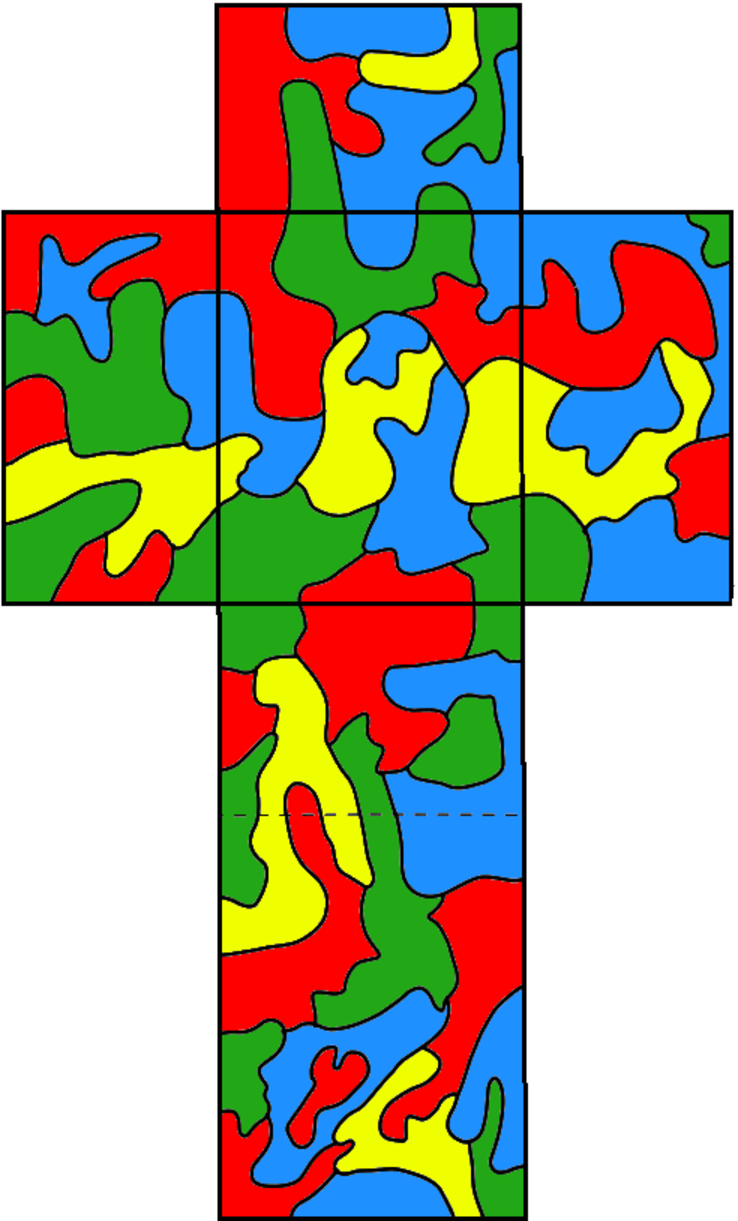
\includegraphics[width=8cm]{../../S23_Representer_le_pave_et_le_cylindre/Images/Pave_4_couleurs}}
    \end{center}

\pagebreak


\AAtitre{Séquence 24 : Le puzzle de brousseau}

   Passer de \Lg{4} à \Lg{5} revient (par exemple) à effectuer un agrandissement de coefficient $\dfrac{5}{4} =1,25$. \par
   Il suffit donc de multiplier toutes les longueurs par 1,25.
   \begin{center}
      {\psset{unit=1.25}
      \begin{pspicture}(-1,-1)(12,12)
         \psframe(0,0)(11,11)
         \psframe(4,0)(3.7,0.3)
         \psframe(11,9)(10.7,8.7)
         \psline(4,0)(4,9)(11,2)
         \psline(6,11)(0,5)
         \psline(11,9)(4,9)
         \rput(2,9){\bf\large A}
         \rput(8.5,10){\bf\large B}
         \rput(8.5,7){\bf\large C}
         \rput(2,4){\bf\large D}
         \rput(7,3){\bf\large E}
         \rput{90}(11.5,5.5){\Lg{8,75}}
         \rput{90}(11.5,1){\Lg{2,5}}
         \rput(8.5,11.5){\Lg{6,25}}
         \rput(3,11.5){\Lg{7,5}}
         \rput{90}(-0.5,8){\Lg{7,5}}
         \rput{90}(-0.5,2.5){\Lg{6,25}}
         \rput(2,-0.5){\Lg{6,25}}
         \rput(7.5,-0.5){\Lg{8,75}}
         \rput{90}(3.5,4.5){\Lg{11,25}}
         \rput{90}(11.5,10){\Lg{2,5}}
         \rput(8,8.5){\Lg{8,75}}
      \end{pspicture}}
   \end{center}

\vfill
\pagebreak


\ARtitre{Séquence 24 : Empreinte carbone}
   Pour voir si cette infographie est bien réalisée, il faut vérifier que l'aire de chaque \og bulle \fg{} rectangulaire est proportionnelle au nombre de kilos équivalents CO$_{2}$ émis. \par
   $\bullet$ On peut commencer par vérifier globalement, par domaine. \par
      Dans un tableau, on récapitule les données dont on a besoin : longueur de la bulle, hauteur de la bulle, ce qui nous permet de déterminer son aire. Ensuite, on vérifie qu'il y a proportionnalité entre l'aire et l'émission de CO$_{2}$ en calculant, par exemple, le rapport entre les deux. \par
      \begin{center}
         {\hautab{1.5} \small
         \begin{tabular}{|p{3cm}|*5{C{1.5}|}}
            \hline
            & longueur & hauteur & aire & carbone & rapport \\
            \hline
            Transport & 8,3 & 6,9 & 57,27 & 2650 & 46,3 \\
            \hline
            Alimentation & 8,3 & 6,1 & 50,63 & 2350 & 46,4 \\
            \hline
            Habitat & 4,4 & 9,4 & 41,36 & 1900 & 45,9 \\
            \hline
            Consommation & 3,6 & 9,4 & 33,84 & 1600 & 47,3 \\
            \hline
            Dépenses pub. & 8,1 & 3,2 & 25,92 & 1400 & 46,7 \\
            \hline
         \end{tabular}}
      \end{center}
      Les rapports sont situés autour de 46-47, on peut donc en déduire que les bulles de domaines sont bien proportionnées (les différences sont dues aux approximations de lecture des grandeurs). \medskip
   
   $\bullet$ On peut ensuite par vérifier si, par domaine, les bulles détails sont bien réalisées. \par
      On crée le même type de tableau, par exemple pour le domaine des transports :
      \begin{center}
         {\hautab{1.5} \small
         \begin{tabular}{|p{3cm}|*5{C{1.5}|}}
            \hline
            & longueur & hauteur & aire & carbone & rapport \\
            \hline
            Voiture & 6,3 & 6,9 & 43,47 & 2030 & 46,7 \\
            \hline
            Avion & 1,9 & 4,8 & 9,12 & 430 & 47,1 \\
            \hline
            Autres & 1,9 & 2,1 & 3,99 & 190 & 47,6 \\
            \hline
         \end{tabular}}
      \end{center}  
   Les rapports sont situés autour de 47 également, on peut donc en déduire que les bulles de détails sont bien proportionnées. \medskip
   
   \cor{En conclusion, on peut légitimement émettre l'hypothèse que le reste de l'infographie est construire sous le même modèle, et donc que cette infographie a les bonnes proportions}.

\vfill


\AAtitre{Séquence 25 : Je veux du chocolat !}
   
   \begin{enumerate}
       \item Calcul 1 : $20\times\Masse{64}+20\times\Masse{32} =\Masse{1280}+\Masse{640} =\cor{\Masse{1920}}$. \par
           Calcul 2 : $\Masse{64}+\Masse{32} =\Masse{96}$ et $20\times\Masse{96} =\cor{\Masse{1920}}$.
       \item Calcul 1 : $35\times\Masse{56}+35\times\Masse{40} =\Masse{1960}+\Masse{1400} =\cor{\Masse{3360}}$. \par
           Calcul 2 : $\Masse{56}+\Masse{40} =\Masse{96}$ et $35\times\Masse{96} =\cor{{3360}}$.
       \item 
           \begin{enumerate}
               \item Calcul 1 : $a\times x+b\times x =ax+bx$ \par
                   Calcul 2 : $(a+b)\times x =(a+b)x$
               \item $(a+b)x =ax+bx$
           \end{enumerate}
   \end{enumerate}

\pagebreak


\ARtitre{Séquence 25 : Un diamant littéral}
   
    \begin{center}  
        {\psset{unit=2.5}
        \begin{pspicture}(-0.107,0)(6,8)      
            \rput{-60}(2,4){\tri{7x+70x}{x}{154x}} %2
            \rput(2,4){\tri{14x-35x+22x}{49x}{7x+35x}} %1
            \rput{60}(2,4){\car{14x+35x}{13x}{}{4x-8x+6x}} %6
            \rput{150}(2,4){\tri{2x}{20x+5x}{}} %12
            \rput{-150}(2,4){\car{25x}{}{20x+8x-5x}{77x}} %5
            \rput{-150}(3,2.27){\tri{23x}{10x+20x}{}} %11
            \rput{-90}(3,2.27){\tri{30x}{10x+10x}{}} %10
            \rput{-120}(4,4){\car{14x+140x}{20x}{}{10x+5x}} %4
            \rput{-30}(4,4){\tri{15x}{16x-4x}{}} %9
            \rput{30}(4,4){\car{12x}{}{8x-4x}{42x}} %3
            \rput{30}(3,5.73){\tri{4x}{2x-2x}{}} %8
            \rput{90}(3,5.73){\tri{0}{2x+15x-4x}{}} %7
        \end{pspicture}}
    \end{center}

\vfill
\pagebreak

\AAtitre{Séquence 26 : Des droites concourantes}

    \begin{enumerate}
        \item
            \begin{itemize}
                \item Tracer des arcs de cercle de même rayon de centre $M$ et $N$ ;
                \item relier les points d'intersection des arcs de cercle : il s'agit de la médiatrice du segment $[MN]$.
            \end{itemize}
        \item La médiatrice d'un segment est \cor{la droite perpendicualaire à ce segment et passant par le milieu du segment}.
        \item \cor{Tout point de la médiatrice d'un segment est à égale distance des deux extrémités du segment}.
        \item Tracer la médiatrice de tous les côtés de ces deux polygones.
            \begin{center}
                {\psset{unit=0.8}
                \begin{pspicture}(0.5,-2)(20,6.5)
                    \pstGeonode[CurveType=polygon,PointName=none,PointSymbol=none](0,2){A}(6,0){B}(9,3){C}
                    \pstGeonode[CurveType=polygon,PointName=none,PointSymbol=none](12,0){J}(20,1){K}(16,5){L}(12,3){M}
                    \psset{CodeFig=true,PointName=none,PointSymbol=none,nodesepA=-1}
                    \pstMediatorAB[CodeFigColor=DodgerBlue,nodesepB=-2.2]{A}{B}{D}{E}
                    \pstMediatorAB[CodeFigColor=Crimson,nodesepB=-3.2]{B}{C}{F}{G}
                    \pstMediatorAB[CodeFigColor=ForestGreen,nodesepA=-2.9]{C}{A}{H}{I}
                    \pstMediatorAB[CodeFigColor=DodgerBlue,nodesepB=-2]{J}{K}{O}{P}
                    \pstMediatorAB[CodeFigColor=Crimson,nodesepB=-2.5]{K}{L}{Q}{R}
                    \pstMediatorAB[CodeFigColor=ForestGreen,nodesepB=-2.8]{L}{M}{S}{T}
                    \pstMediatorAB[CodeFigColor=DarkOrange,nodesepB=-5]{M}{J}{U}{V}
                \end{pspicture}}
            \end{center}
        \item Les médiatrices sont concourantes \cor{pour le triangle}.
        \item Dessin tracé au fur et à mesure :
            \begin{center}
                \begin{pspicture}(-1,0)(6,4)
                    \psset{CodeFig=true,PointSymbol=none,linecolor=Crimson}
                    \pstTriangle{A}(5,0){B}(1.5,3){C}
                    \pstCircleABC[RightAngleSize=0.2,CodeFigColor=black]{A}{B}{C}{O}
                \end{pspicture}
            \end{center}
        \item \cor{$OA =OB$}.
        \item \cor{$OB =OC$}.
        \item \cor{$OA =OB = OC$}.
        \item Le point $O$ est \cor{sur la médiatrice de $[CA]$}.
        \item Le cercle de centre $O$ passant par $A$ \cor{passe par les trois sommets $A, B$ et $C$ du triangle}.
        \item \cor{Les trois médiatrices d'un triangles qont concourantes} en un point $O$ qui est le centre du cercle circonscrit au triangle.
    \end{enumerate}

\vfill


\ARtitre{Séquence 26 : La droite d'Euler}

    \begin{enumerate}
    \setcounter{enumi}{4}
    \item $H, O$ et $G$ sont confondus lorsque \cor{le triangle $ABC$ est équilatéral}.
    \item On peut conjecturer que \cor{les points $H, O$ et $G$ sont alignés}.
    \item On peut conjecturer que \cor{$OH =3\,OG$}.
    \end{enumerate}

\pagebreak


\AAtitre{Séquence 27 : La formule de Pick}
    
    \begin{enumerate}
        %\setenumerate{enumi}{3}
        \item On obtient \cor{des parallélogrammes}.
        \item Les parallélogrammes \cor{ont tous la même aire}, puisqu'ils sont tous formés à partir du même rectangle.
        \item L'aire du parallélogramme s'obtient en \cor{multipliant la longueur de la base par sa hauteur}.
    \end{enumerate}

\vfill


\ARtitre{Séquence 27 : L'aire du parallélogramme}
        
        \begin{enumerate}
            \item $\mathcal{A}_{PICK} =6\,u.\ell.\times4\,u\ell. =\cor{24\,u.a.}$
            \item $\mathcal{A}(MOFE) =5\,u.\ell.\times5\,u.\ell. =25\,u.a.$ \par \smallskip
                $\mathcal{A}(MOR) =\dfrac{5\,u.\ell.\times4\,u.\ell.}{2} =10\,u.a.$ \par \smallskip
                $\mathcal{A}(MULE) =4\,u.\ell.\times3\,u.\ell.+\dfrac{4\,u.\ell.\times2\,u.\ell.}{2} =16\,u.a.$ \par \smallskip
                En sommant, on obtient : $\mathcal{A}(FORMULE) =25\,u.a.+10\,u.a.+16\,u.a. =\cor{51\,u.a.}$ \smallskip
            \item \cor{$i =18$} et \cor{$b =14$} donc, $\mathcal{A} =18+\dfrac{14}{2}-1 =\cor{24}$. \smallskip
            \item \cor{$i =41$} et \cor{$b =22$} donc, $\mathcal{A} =41+\dfrac{22}{2}-1 =\cor{51}$. \smallskip
            \item On décompose comme à la question 2.
                \begin{itemize}
                    \item MOFE : $i =16$, $b =20$, $\mathcal{A} =16+\dfrac{20}{2}-1 =25$. \smallskip
                    \item MOR : $i =7$ et $b =8$, $\mathcal{A} =7+\dfrac{8}{2}-1 =10$. \smallskip
                    \item MULE : $i =10$ et $b =14$, $\mathcal{A} =10+\dfrac{14}{2}-1 =16$. \smallskip
                    \item FORMULE : $\mathcal{A} =25+10+16 =51$. \par
                        \cor{La somme des résultats obtenus est égale au résultat trouvé à la question 2.}
            \end{itemize}
        \end{enumerate}

\vfill


\AAtitre{Séquence 28 : Propriétés des symétries}

    \begin{enumerate}
        \item[2.] On a \cor{$AD =A'D'$}.
        \item[3.] On a \cor{$\widehat{ABC} =\widehat{A'B'C'}$}.
        \item[4.] Le point $E'$ ets situé \cor{sur la droite $(A'B')$}.
        \item[5.] \cor{oui, deux droites parallèles dans la figure d'origine restent parallèles  dans la figure symétrique}.
        \item[7.] On a \cor{$BC =B'C'$}.
        \item[8.] On a \cor{$\widehat{ACDEC} =\widehat{C'D'E'}$}.
        \item[9.] Le point $F'$ ets situé \cor{sur la droite $(A'B')$}.
        \item[10.] \cor{oui, deux droites parallèles dans la figure d'origine restent parallèles  dans la figure symétrique}.
    \end{enumerate}
    
\pagebreak


\ARtitre{Séquence 28 : Entrelacs chinois}

    \begin{center}
        {\psset{unit=0.9}
        \begin{pspicture}(0,0)(17,19.3)
            \psgrid[subgriddiv=0,gridlabels=0,gridcolor=lightgray](0,0)(17,19)
            \psline[linecolor=RoyalBlue](8.5,0)(8.5,19)
            \psline[linecolor=RoyalBlue](0,9.5)(17,9.5)
            \psset{doublesep=7mm,linewidth=1mm,doubleline=true,doublecolor=Green!35}
                \psline(0.5,0)(0.5,4.5)(16.5,4.5)(16.5,0.5)(9.5,0.5)(9.5,18.5)(16.5,18.5)(16.5,14.5)(0.5,14.5)(0.5,18.5)(7.5,18.5)(7.5,14.5)(7.5,0.5)(0,0.5)
                \pscircle[doublecolor=IndianRed](8.5,9.5){3}
                \pscircle[doublecolor=DarkOrange](8.5,9.5){7}
                \psline(7.5,1)(7.5,9.5)
                \psline(7.5,14)(7.5,15)
                \psline(9.5,18)(9.5,9.5)
                \psline(9.5,5)(9.5,4)
                \psline(9,14.5)(10,14.5)
                \psline(1,14.5)(7,14.5)
                \psline(7,4.5)(8,4.5)
                \psline(10,4.5)(16,4.5)
            \psline[doubleline=false,linewidth=1mm](0.05,1)(0.05,0.05)(1,0.05)
        \end{pspicture}}
    \end{center}